% !TeX spellcheck = en_GB
\documentclass[10pt,letterpaper,oneside]{article}
\usepackage{fontspec}
\usepackage{arev}
\usepackage[utf8]{inputenc}
\usepackage[T1]{fontenc}
\usepackage{amsmath}
\usepackage{amsfonts}
\usepackage{amssymb}
\usepackage{graphicx}
\usepackage{csquotes}
\usepackage{booktabs}
\usepackage{multicol}
\usepackage{enumerate}
\usepackage{microtype}
\usepackage[labelfont=bf,font={small}]{caption}
\usepackage{hyperref}
\usepackage{booktabs}
\usepackage{subcaption}
\usepackage{fancyhdr}
\usepackage[svgnames]{xcolor}
\usepackage{mdframed}
\usepackage{multicol}
\usepackage[para]{footmisc}
\usepackage{siunitx}
\usepackage{cleveref}
\usepackage{listings}
\usepackage{cprotect}


\lstset{ % General setup for the package
	language=Python,
	basicstyle=\small\ttfamily,
	tabsize=4,
	columns=fixed,
	showstringspaces=false,
	showtabs=false,
	keepspaces,
	commentstyle=\color{SeaGreen},
	keywordstyle=\bf\ttfamily\color{DarkBlue},
	stringstyle=\ttfamily\color{Crimson}
}

\newfontfamily\symbolfont{Symbola}
\usepackage[left=1in,right=1in,top=1in,bottom=1in,marginparwidth=0.3in]{geometry}

\usepackage[sorting=none]{biblatex}
\addbibresource{../bibliography.bib}

\ifx\NoteAuthor\undefined
  \def\NoteAuthor{Andreas Stöckel and Chris Eliasmith}
\fi

\ifx\BasedOn\undefined
  \def\BasedOn{Based on lecture notes by\\Chris Eliasmith and Terrence~C.~Stewart}
\fi

\author{\NoteAuthor\\[0.5cm]\BasedOn}
\newcommand{\baseCodeURL}{https://github.com/celiasmith/syde556-f23/blob/master/lectures}

\fancyhf{}
\fancyhead[L]{SYDE 556/750 Lecture Notes}
\fancyhead[R]{\NoteAuthor}
\fancyfoot[C]{\thepage}
\pagestyle{fancy}

\setlength{\parindent}{0em}
\setlength{\parskip}{0.5em}
\renewcommand{\baselinestretch}{1.25}

\renewcommand{\vec}[1]{{\mathbf{#1}}}
\newcommand{\mat}[1]{{\mathbf{#1}}}
\newcommand{\T}{\ensuremath{\mathrm{T}}}
\renewcommand{\epsilon}{\varepsilon}
\renewcommand{\phi}{\varphi}

\makeatletter
\newcommand{\superimpose}[2]{%
	{\ooalign{{#1}\hidewidth\cr{#2}\hidewidth\cr}}}
\makeatother
\newcommand{\SolidCircle}[2]{\superimpose{\color{#1}\symbolfont ⬤}{\textbf{\color{white}#2}}\hspace{1em}}
\newcommand{\OPlus}{\SolidCircle{DarkGreen}{\kern0.75pt+}}
\newcommand{\OMeh}{\SolidCircle{DarkOrange}{~}}
\newcommand{\OMinus}{\SolidCircle{DarkRed}{\kern2.25pt--}}

\newcommand{\YouTube}[2][Video]{\href{https://youtu.be/#2}{{\symbolfont 📺}~{#1}}%
%\footnote{\url{https://youtu.be/#2}}%
}

\newcommand{\CodeLink}[2][Code]{\href{\baseCodeURL/#2}{{\symbolfont ⌨}~\emph{#1}}}

\newcommand{\MakeTitle}[1]{
\maketitle
\begin{center}
	
\includegraphics[width=0.5\textwidth]{../assets/uwlogo.pdf}\\[1cm]
	{#1}\
\end{center}

\vfill

\thispagestyle{empty}
\setcounter{page}{0}
\newpage

\pagenumbering{roman}
\setcounter{tocdepth}{2}
\tableofcontents
\newpage

\setcounter{page}{0}
\pagenumbering{arabic}}

\reversemarginpar


\newcommand{\ColorBox}[3]{%
	\marginpar{%
		\huge\raisebox{-3ex}{\symbolfont{#1}}%
	}%
	\begin{mdframed}[hidealllines=true,backgroundcolor=#2,innertopmargin=0.25cm,innerbottommargin=0.25cm]%
		{#3}
	\end{mdframed}}

\newcommand{\Note}[1]{\ColorBox{📌}{WhiteSmoke}{\textbf{Note:} #1}}
\newcommand{\Example}[1]{\ColorBox{💡}{WhiteSmoke}{\textbf{Example:} #1}}
\newcommand{\Aside}[1]{\ColorBox{🌟}{WhiteSmoke}{\emph{Aside:} #1}}
\newcommand{\Python}[1]{\ColorBox{🐍}{WhiteSmoke}{#1}}
\newcommand{\Notation}[1]{\ColorBox{\huge$\Sigma$}{WhiteSmoke}{\textbf{Notaton:} #1}}

\newcommand{\ConstructionSite}{\hrulefill {\symbolfont 🚧} UNDER CONSTRUCTION {\symbolfont 🚧} \hrulefill}

\newenvironment{ImportantEqn}[1]{\mdframed\raggedleft\emph{({#1})}\align}{\endalign\endmdframed}

\date{March 31, 2020}
\title{SYDE 556/750 \\ Simulating Neurobiological Systems \\ Lecture 12: Biological Details}

\newcommand{\Pred}[1]{\ensuremath{\mathbf{\textcolor{Crimson}{#1}}}}
\newcommand{\Obj}[1]{\ensuremath{\mathtt{\textcolor{RoyalBlue}{#1}}}}
\newcommand{\Fun}[1]{\ensuremath{\mathit{\textcolor{ForestGreen}{#1}}}}
\newcommand{\CC}{\circledast}

\begin{document}

\MakeTitle{Accompanying readings: Stöckel and Eliasmith, 2019 \cite{stockel2019passive}}

\section{Introduction}

\Note{Within the Neural Engineering Framework, we are making some \enquote{biologically implausible} assumptions. In this lecture, we discus some of these assumptions and present ways to build networks that incorporate more biological detail.}

Biology puts a few more constraints onto neural networks than what we assumed when deriving the equations underlying the NEF principles. The following list discusses three particular constraints we ignored. We will discuss how to extend the NEF to take these restrictions into account, resulting in potentially more biologically plausible networks.
\begin{itemize}
	\item \textbf{Dale's principle: Neurons are either excitatory or inhibitory.} In biology, each type of neuron can only produce one type of neurotransmitter \cite{strata1999dale}. Most neurotransmitters have either an excitatory or inhibitory effect on the post-neuron. This effectively means that \emph{neurons}, not individual synapses, are either excitatory or inhibitory. However, when looking at synaptic weight matrices $\mat W$ computed within the NEF, one will find that individual pre-neurons $j$ are both connected excitatorily  and inhibitorily to post-neurons (i.e., for some post-neuron $i$, $w_{ij} > 0$, while for another post-neuron $i'$, $w_{i'j} < 0$).
	\item \textbf{No bias currents.} We assumed that each neuron $i$ possesses a bias current $J^\mathrm{bias}_i$. While this may be seen as a model for the excitability of a neuron (neurons with small $J^\mathrm{bias}_i$ need larger input currents), bias currents in the literal sense do not exist in biology.
	\item \textbf{Conductance-based synapses: Post-synaptic currents are not linear.} We defined the post-synaptic current $J_i$ as a linear combination of pre-synaptic activities. If two spikes arrive from a pre-neuron, the total post-synaptic current evoked by these pre-activities will just be the sum of the individual pre-activities. This assumption is also called \enquote{current-based synapses}, i.e., we are assuming that each synapse is generating a current that is injected into the neuron. Better models of synapses are \emph{conductance-based}, where the amount of current injected into the neuron depends on the momentary membrane potential. This phenomenon can be exploited to compute non-linear multivariate functions without having to represent all variables in the pre-population.
\end{itemize}
Of course, we made several other modelling assumptions that we do not discuss here. For example, when deriving the dynamics principle, we assumed that the synaptic filter dominates the overall neural dynamics. This is not necessarily true in biology. The neuron itself may have dynamical properties with time-constants significantly longer than the synaptic filter.

\Note{\emph{The NEF and biological detail.} As we have discussed several times before, the goal of the NEF is not to build the most biologically realistic network models, but to bridge the gap between neurobiology and behavioural/cognitive models. Correspondingly, extensions to the NEF should either provide a way to incorporate important neurobiological constraints  into models (such as Dale's principle), or help explaining higher-level phenomena (such as dedritic computation using conductance-based synapse models).}


\section{Taking Dale's Principle Into Account and Eliminating Bias Currents}

Brain microcircuits mapped out by neurobiologists often distinguish between \enquote{excitatory} and \enquote{inhibitory} neuron populations. As discussed above, according to Dale's principle, individual neurons can only produce one type of neurotransmitter. Since the effect on the post-neuron (i.e., whether it is excited or inhibited) is mostly determined by the neurotransmitter type, neurons tend to affect their post-neurons either  excitatorily or inhibitorily.

With the techniques we have discussed in the lecture so far, it is unclear how to incorporate this constraint into NEF networks. In other words, it is unclear how to force all synaptic weights $w_{ij}$ of a particular pre-neuron $j$ (i.e., columns in the weight matrix $\mat W$) to be either positive or negative. This makes it harder to build models of the aforementioned brain microcircuits.

\Note{\emph{Representation space and synaptic weights.} Remember that we distinguish between the representational space and the neural activity space in the NEF.

Suppose that we wanted to inhibit the post-neuron population, i.e., have synaptic connections $w_{ij}$ that are either zero or negative.
Computing an \enquote{inhibitory} function in \emph{representation space} such as $f(x) = -x$ does not imply that the neurons in the post ensemble are less active than the neurons in the pre-population (assuming positive $x$)!

This is partially due to the fact that we typically have \enquote{positive} and \enquote{negative} encoders in the post-population. Some neurons in the post-population will be more active (i.e., will be excited) when representing smaller values.

Generally speaking, the algebraic sign of the synaptic weights $w_{ij}$ depends on the signs of \emph{both} the decoders $\mat D$ and the encoders $\mat E$. Under some circumstances we can choose neural tuning curves of the pre- and post-ensemble in such a way that---depending on the function we compute---weights will be mostly positive or negative. However, ensuring this tends to be quite tricky. The method we discuss in the following is much simpler, although not directly implemented in Nengo.}

\subsection{Solving for weights in current space}

We can incorporate Dale's principle quite easily into NEF networks if we solve for full connection weight matrices $\mat W$ in \enquote{current space}.  Solving for \enquote{full connection weight matrices} $\mat W$ means that we can no longer use the factorization trick $\mat W = \mat E \mat D$ when simulating our networks, since we never solve for decoders $\mat D$ in the first place, but directly for $\mat W$ instead.

In particular, we solve for the synaptic weights of a single post-neuron $i$. That is, we compute each row $\vec w_i$ of the weight matrix $\mat W$ individually. According to the \enquote{current-based synapse} model \cite{roth2009modeling}, the static (i.e., not taking the synaptic filter into account) post-synaptic current $\hat J_i$ of a post-neuron $i$ given the pre activity $\vec a(\vec x)$ of a pre-population representing the value $\vec x$ is
\begin{align}
\hat J_i &= \langle \vec a(\vec x), \vec w_i \rangle \,.
\label{eqn:j_input}
\end{align}
Furthermore, we have a \emph{normative constraint} from the encoding equation that tells us what input current a neuron should receive if the entire population represents a value $\vec x$:
\begin{align}
J_i &= \alpha_i \langle \vec x, \vec e_i \rangle + J^\mathrm{bias}_i \,.
\label{eqn:j_target}
\end{align}
\Note{Here, \emph{normative constraint} means that, when building a NEF network, we choose parameters $\alpha_i$, $\vec e_i$, $J^\mathrm{bias}_i$ that determine what current \emph{we would like} each individual neuron to receive, if its population as a whole represents a value $\vec x$. With the method below we solve for connection weights $\vec w_i$ that approximately compute the current in \cref{eqn:j_target} by linearly decoding the pre-population activities.}
When implementing the NEF principle two, i.e., computing a function $f$ in the connection between two ensembles, we need to minimize the error $(\hat J_i - J_i)^2$, i.e., we need to make sure that the actual input current $\hat J_i$ is equal to the desired input current $J_i$. Combining \cref{eqn:j_input} and \cref{eqn:j_target} for $N$ samples results in the following optimization problem:
\begin{align}
	\vec w_i &= \arg\min_{\vec w_i} \sum_{k = 1}^N \left( \big\langle \vec a(\vec x_k), \vec w_i \big\rangle - \alpha_i \big\langle \vec f(x_k), \vec e_i \big\rangle + J^\mathrm{bias}_i \right)^2 \,.
	\label{eqn:opt_linear}
\end{align}
We can write this in matrix form as
\begin{align*}
	\vec w_i &= \arg\min_{\vec w_i} \big\| \mat A \vec w_i - \mat J^\mathrm{tar} \big\|^2 \,,
\end{align*}
which can be solved using a least-square solver, as we have discussed multiple times before.

Notice that using the resulting weights will approximately evoke the desired target current $J_i$ defined in \cref{eqn:j_target} in the post neuron. This includes the bias current $J^\mathrm{bias}_i$, the gain $\alpha_i$, as well as the encoder $\vec e_i$. Correspondingly, after solving for weights, the entire network is solely governed by \cref{eqn:j_input}. While the neuron parameters $J^\mathrm{bias}_i$, $\alpha_i$, $\vec e_i$ are still used to control the tuning curves of our neural population (i.e., to establish the \enquote{normative constraint}, see above), these parameters are no longer part of our simulation. We no longer have to assume that each neuron possesses a bias current $J^\mathrm{bias}_i$, this current is implicitly decoded from the pre-population---we have \enquote{eliminated the bias current}.

\Note{\emph{The current translation function.} The function that translates a represented value $\vec x$ into a current $J_i$ is called \enquote{current translation function}. So far, we generally chose the affine function given in \cref{eqn:j_target}, i.e.,
\begin{align*}
	J_i(\vec x) &= \alpha_i \langle \vec x, \vec e_i \rangle + J^\mathrm{bias}_i \,.
\end{align*}
However, note that this function is arbitrary. With the technique detailed above, i.e., solving for weights in current space, we can choose \emph{any} current translation function, and, as a result, \emph{any} tuning curve shape, as long as this function can be decoded from the pre-population. Since decoding affine functions tends to be possible with a small error (see the lecture on analysing representations), this is a sane default.}

\subsection{Enforcing Dale's Principle}

In a sense, the above method of solving for a synaptic weight matrix $\vec W$ is a reformulation of the decoder computation problem. Instead of computing a single function decoder for the entire post-population, we compute a \enquote{current decoder} for each post-neuron. While this allows us to eliminate the bias current from the post-population---since it is implicitly computed as part of the \enquote{current decoders}---we are still not taking Dale's principle into account. Luckily, since we now solve for weights directly, this has become much easier.

Consider the general case of the pre-population being split into a set of excitatory and inhibitory neurons. Note that these sets could also be empty, corresponding to the entire neuron population being purely excitatory or inhibitory. Correspondingly, we now have two separate sets of connections: excitatory connections with corresponding weights $\vec w_i^+$, and inhibitory connections with the corresponding weights $\vec w_i^-$. We can now rewrite the optimization problem from \cref{eqn:opt_linear} as
\begin{align}
	\vec w_i^+, \vec w_i^- &= \arg\min_{\vec w_i^+, \vec w_i^-} \big\| \mat A^+ \vec w^+_i - \mat A^- \vec w^-_i - \mat J^\mathrm{tar} \big\|^2 \,, & \text{with respect to} \quad \vec w_i^+, \vec w_i^- \geq 0 \,.
	\label{eqn:opt_dale}
\end{align}
where $\mat A^+$ and $\mat A^-$ are the activities of the excitatory and inhibitory pre-neurons. Rearranging this equation yields
\begin{align*}
	\vec w'_i &= \big(\vec w^-_i, \vec w^+_i\big) 
		       = \arg\min_{\vec w_i} \big\| \big( \mat A^+, -\vec A^- \big) \big(\vec w^-_i, \vec w^+_i \big)^\T - \mat J^\mathrm{tar} \big\|^2
		       = \arg\min_{\vec w_i} \big\| \mat A' \big(\vec w'_i\big)^\T - \mat J^\mathrm{tar} \big\|^2 \,, \\
	\text{w.r.t. } \vec w'_i &\geq 0 \,.
\end{align*}
This problem is called \emph{non-negative least squares} (NNLS), and can, for example, be solved using the SciPy function \texttt{scipy.optimize.nnls}.

Using this method, we declare each neuron within an NEF network to be either excitatory or inhibitory, and then solve for connection weight matrices that take this constraint into account. As demonstrated below, depending on the function we are computing, the impact of doing this with respect to the precision is negligible, although there are some idiosyncrasies one has to keep in mind when building networks in this way, particularly the fact that not all functions can be decoded from the pre-activities using purely excitatory/inhibitory weights.

\Note{\emph{Multiple pre-populations.} When using the above methods for building networks with multiple pre-populations targeting the same post-population, the bias current must not be decoded from multiple pre-populations at once. There are several ways to accomplish this. For example, when receiving input from $n$ pre-populations, one can just solve for $\frac{1}n$ of the bias in each connection.

Another method is to \enquote{stack} all pre-population activities into a single vector $\vec a$ to form a \enquote{virtual} pre-population, and to compute all connection weights at once. This implicitly distributes the bias current among the individual connections and is exactly the method implemented by \texttt{nengo-bio} (see below).}

\subsection{Biologically plausible Nengo networks using \texttt{nengo-bio}}

\begin{figure}
	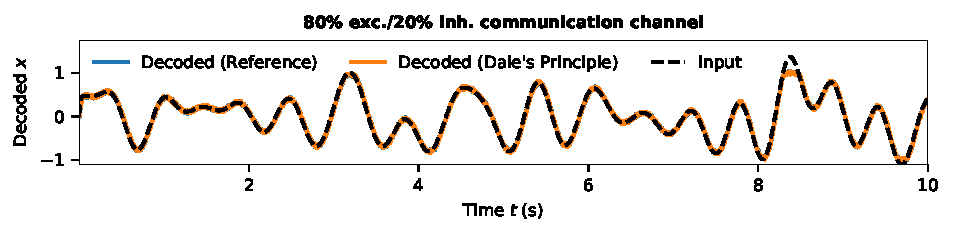
\includegraphics{media/nengo_bio_communication_channel.pdf}
	\caption{Two communication channels: one using standard (reference) NEF methodology, and one using a pre-population with 80\% excitatory neurons and 20\% inhibitory neurons. When computing the identity function, there is virtually no loss in accuracy when accounting for Dale's principle. \CodeLink{lecture_12/media/code/nengo_bio_experiments.ipynb}}
	\label{fig:nengo_bio_communication_channel}
\end{figure}

While we could manually solve for connection weight matrices $\mat W$ using the above method and use the resulting connection weight matrices in a \enquote{neurons-to-neurons} connection in Nengo, this tends to be quite tedious. An easier way is to use the \texttt{nengo-bio}\footnote{See \url{https://github.com/astoeckel/nengo-bio}} library, an (experimental) free software library extending Nengo to facilitate the construction of biologically (more) plausible neural networks.

\paragraph{Example: An 80\% excitatory/20\% inhibitory communication channel}
The following code in \texttt{nengo-bio} implements a communication channel from a neuron population with 80\% excitatory neurons and 20\% inhibitory neurons. This is approximately the ratio of excitatory to inhibitory neurons found in cerebral cortex.
\cprotect\Python{\begin{lstlisting}[morekeywords={with,as}]
import nengo
import nengo_bio as bio

with nengo.Network(seed=4909) as model:
    nd_in = nengo.Node(nengo.processes.WhiteSignal(
       rms=0.5, high=2.0, period=10.0))

    # Use "bio.Ensemble" objects
    ens_a = bio.Ensemble(n_neurons=101, dimensions=1, p_exc=0.8) # 80% excitatory
    ens_b = bio.Ensemble(n_neurons=102, dimensions=1)

    # Use a nengo.Connection to connect nodes or "normal"
    # nengo.Ensemble objects to a bio.Ensemble
    nengo.Connection(nd_in, ens_a)

    # Use bio.Connection for connections between bio.Ensemble objects
    bio.Connection(ens_a, ens_b)
\end{lstlisting}}
The result of running this code is shown in \cref{fig:nengo_bio_communication_channel}.  Restricting the excitatoriness or inhibitoriness of the pre-neurons does not have a visible impact on the accuracy of the system. In fact, the communication channel will still work fine, even for 100\% excitatory pre-neurons or 100\% inhibitory pre-neurons (given that there is a suitable bias source). Depending on the pre-population tuning curves, the error may increase for more complex functions.

\begin{figure}
	\centering
	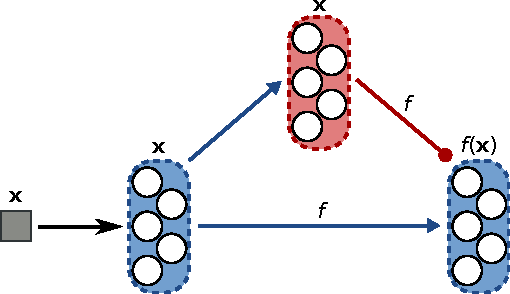
\includegraphics{media/inhibitory_interneuron_network.pdf}
	\caption{Example of a network with inhibitory interneurons. An excitatory signal is relayed via an inhibitory population of neurons. Blue lines correspond to purely excitatory connections, red lines to purely inhibitory connections. Assuming that both the original neuron population and the interneuron population represent the same value, we can compute a function $f$ across two separate sets of connections.}
	\label{fig:inhibitory_interneuron_network}
\end{figure}
\paragraph{Example: Inhibitory Interneurons}
\Cref{fig:inhibitory_interneuron_network} depicts a connectivity scheme that is often found in brain microcircuits. A signal $\vec x$ is relayed from a purely excitatory pre-population via both a direct connection and a population of inhibitory interneurons. Assuming that both pre-populations represent the same value, we can still compute arbitrary functions $f$ across both the excitatory and inhibitory connection. \texttt{nengo-bio} comes with a special syntax for this:
\cprotect\Python{\begin{lstlisting}[morekeywords={with,as}]
import nengo
import nengo_bio as bio

with nengo.Network(seed=4909) as model:
    nd_in = nengo.Node(nengo.processes.WhiteSignal(
        rms=0.5, high=2.0, period=10.0))

    ens_a = bio.Ensemble(n_neurons=80, dimensions=1, p_exc=1.0)
    ens_b = bio.Ensemble(n_neurons=20, dimensions=1, p_inh=1.0)
    ens_c = bio.Ensemble(n_neurons=100, dimensions=1)

    # Communication channel from A to B
    bio.Connection(ens_a, ens_b)

    # Tell nengo-bio that A and B represent the same value using "set notation"
    bio.Connection({ens_a, ens_b}, ens_c, function=lambda x: x**2)
\end{lstlisting}}

\begin{figure}[p]
	\begin{subfigure}{\textwidth}
		\centering
		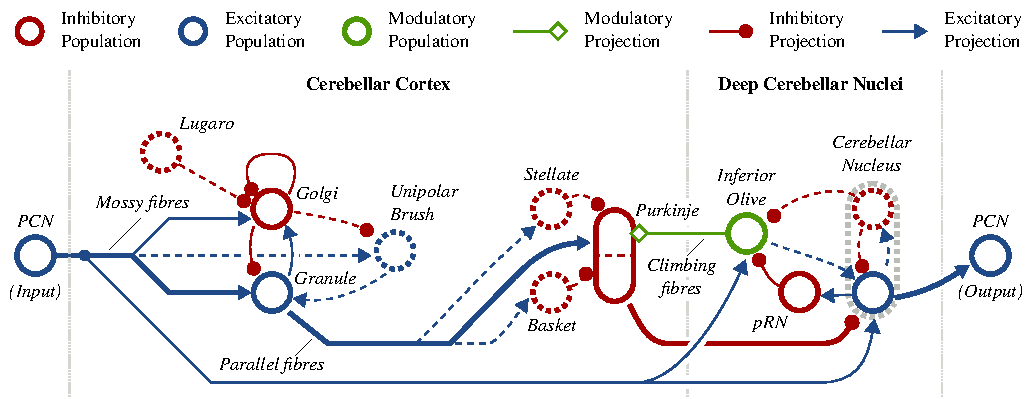
\includegraphics[scale=0.95]{media/cerebellum_anatomy.pdf}
		\caption{The cerebellar microcircuit}
		\label{fig:cerebellum_anatomy}
	\end{subfigure}\\[0.25cm]
	\begin{subfigure}{\textwidth}
		\centering
		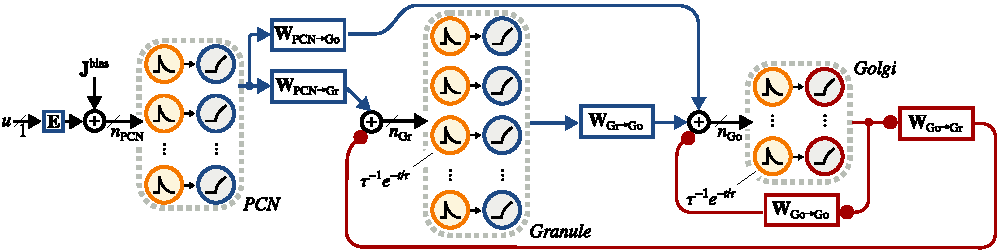
\includegraphics[scale=0.95]{media/delay_network_dale.pdf}
		\caption{A model of the Golgi-Granule circuit}
		\label{fig:delay_network_dale}
	\end{subfigure}\\[0.25cm]
	\begin{subfigure}{\textwidth}
		\centering
		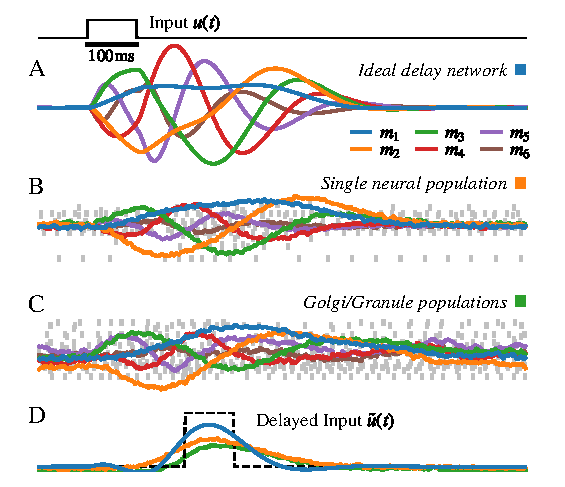
\includegraphics[scale=0.95]{media/delay_network_response.pdf}
		\caption{Diagram showing the delay network response.}
		\label{fig:delay_network_response}
	\end{subfigure}
	\caption{Mapping the delay network onto the Golgi-Granule microcircuit. \textbf{(a)} Depicts the cerebellar microcircuit, the primary pathway is highlighted in bold. Data from \cite{ito2010cerebellar,llinas2010olivocerebellar}. \textbf{(b)} A model of the recurrent Golgi-Granule circuit. Orange circles correspond to the synaptic filters, blue circles to individual neurons. \textbf{(c)} Comparing the Golgi-Granule implementations to other delay network representations.}
\end{figure}
\paragraph{Example: A Model of the Cerebellum}
The cerebellum (Latin for \enquote{little brain}) has long been known in the clinical literature to be important for precise motor control. More recent evidence also points at the cerebellum being important for timing and working-memory related cognitive tasks.

The cerbellar microciruitry is one of the most well-studied of all brain substructures (see \cite{ito2010cerebellar,llinas2010olivocerebellar} for details). To summarize, the cerebellum has a predominantly feed-forward architecture (\cref{fig:cerebellum_anatomy}). Signals from neurons in pre-cerebellar nucleii are routed to a layer of so called \enquote{granule} or \enquote{granular cells}. The granular cells are extremely small (hence the name) and possess only few incoming connections. Astonishingly, about half of all neurons in the human brain are cerebellar granule cells. This means that signals from the PCN are mapped onto a vast number of neurons. Granular cells then connect onto Purkinje cells, which in turn connect to the cerebellar nucleus and from there back to other brain regions. The connections between the Granular and Purkinje cells can be modulated (learned) according to \enquote{error signals} originating from the Inferior Olive.

Marr proposed in 1969 \cite{marr1969theory} that this circuit performs pattern extraction in the granular layer and learns to recombine (decode) the extracted patterns into functions such as corrective motor signals (this is also known as the \enquote{adaptive filter hypothesis}).

One important experiment used to explore cerebellar function is eyeblink conditioning, a form of classical conditioning (see the lecture on learning). The idea is to pair the eyeblink reflex (where a \enquote{puff} of air into the eye, the unconditioned stimulus, causes blinking, the unconditioned response) with a conditioned stimulus, such as a tone. Crucially, the tone precedes the puff by a short duration $t$, typically a few hundred milliseconds. After a while, the person or experimental animal will learn to produce the conditioned response, i.e., will blink even if only the tone is played, while maintaining the original delay. The blink will happen $t$ seconds after the tone. This delayed association is known to be learned by the cerebellum, i.e., the cerebellum is both sufficient and necessary to produce this response.

How exactly the cerebellar microcircuit learns these delays is uncertain. One idea is that the Granule layer somehow produces a temporal function representation, from which the Purkinje cells then decode a delay. While it is---once again---unclear, how exactly this temporal function representation is generated, we have learned in a previous lecture how we can build a spiking neural network that produces such a function representation: the delay network. The granule layer features a set of inhibitory interneurons---the Golgi cells. We could thus try to map the delay network onto this circuit. The resulting circuit is shown in \cref{fig:delay_network_dale}, the response of the circuit compared to more canonical implementations in \cref{fig:delay_network_response}. This circuit can be easily implemented using \texttt{nengo-bio}, taking the excitatoriness and inhibitoriness of individual neuron populations into account.

Note, that in contrast to the standard NEF principle three recurrent architectures, the recurrent connection in the Granular-Golgi subnetwork is through a set of interneurons (the Golgi cells), which potentially changes the dynamics of the system. However, one can mathematically show that exactly the same transformation, i.e., $\mat A' = \tau \mat A + \mat I$ and $\mat B' = \tau \mat B$, must be applied to both recurrent and input connections, respectively.

\section{Conductance-Based Synapses}

\begin{figure}
	\centering
	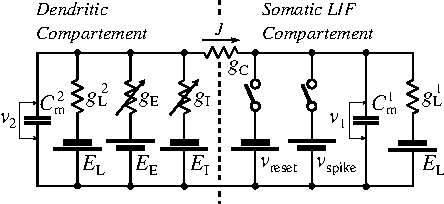
\includegraphics{media/neuron_model.pdf}
	\caption{Two-compartment LIF neuron model with conductance-based synapses. Incoming spikes either increase the conductance of the excitatory channel or the inhibitory channel. In the limit of $g_\mathrm{C} \to \infty$, $v_1(t) = v_2(t)$ this model is equivalent to a single-compartment neuron model.}
	\label{fig:neuron_model}
\end{figure}

We assumed that post-synaptic currents are linear in the pre-synaptic activities, according to the \enquote{current-based} synapse model, which implies that every spike arriving at a specific synapse evokes the same post-synaptic current, independent of the neural state. While this is a good first-order approximation, biology tends to be---as always---a little bit more complicated.

\subsection{The Conductance-Based Synapse Model}

Spikes arriving at a synapse do not directly produce a post-synaptic current. According to Ohm's law, currents $J$ should always be thought of as being evoked by a potential difference $U$ and a conductance $g = 1/R$ that allows charges to flow, i.e., it holds
\begin{align*}
	J &= \frac{U}R = g U \,. && \textit{(Ohm's law)}
\end{align*}

A neurotransmitter arriving at the post-neuron results in ion-channels gated by that neurotransmitter to open. This results in a change in conductance $g$ of the cell-membrane for ions associated with the corresponding ion-channel. Assume that there are $M$ different ion-channels in the neuron. Each of these ion-channels has an associated \enquote{reversal potential $E_\ell$}. The \enquote{conductance-based} synapse model assumes that the conductance for a particular channel $\ell$ is linear in the pre-synaptic activities $\vec a^\ell$ of neurons connected to that channel, and that the current $J$ is the product of the conductance and the difference between the membrane potential $v(t)$ and the specific channel reversal potential $E_\ell$:
\begin{ImportantEqn}{Conductance-Based Synapse Model}
	g_\ell(t) &= \big(\langle \vec a^\ell(\vec x), \vec w_\ell \rangle \ast h_\ell \big) \,, &
	J(t) &= \sum_{\ell=1}^M g_\ell(t) \big( E_\ell - v(t) \big) \,.
\end{ImportantEqn}
The current $J(t)$ is now no longer linear in the pre-synaptic activities---the current depends on the membrane potential $v(t)$, which in return is influenced by the current $J(t)$ according to the neural dynamics. An equivalent circuit diagram for a two-compartment neuron model with conductance-based synapses is depicted in \cref{fig:neuron_model}.

\subsection{Incorporating Synaptic Nonlinearities Into the NEF}

As detailed above, the current-based synapse model in \cref{eqn:j_input} assumes that the post-synaptic current $J$ is a linear combination of the pre-synaptic activities $\vec a$. If we assume separate excitatory and inhibitory input \enquote{channels}, we can rewrite this equation in terms of a function $H$---the \enquote{synaptic nonlinearity model}---that combines these two kinds of inputs, or  \enquote{channel states}. In the case of the current-based synapse model, $H$ is given as
\begin{align}
	\hat J_i &= H\big(\langle \vec a^+, \vec w_i^+ \rangle, \langle \vec a^-, \vec w_i^- \rangle \big) = \langle \vec a^+, \vec w_i^+ \rangle - \langle \vec a^-, \vec w_i^- \rangle \,,
	\label{eqn:H_cur}
\end{align}
i.e., the \enquote{excitatory} inputs produce a positve, the \enquote{inhibitory} inputs a negative current.

When incorporating more complex synapse models into the NEF, the idea is to just use an appropriate function $H(g_1, \ldots, g_M)$ that (nonlinearly) maps channel states (e.g., conductances) onto a current $\hat J_i$. We can then obtain synaptic weights by solving a more complex optimization problem similar to \cref{eqn:opt_linear}
\begin{align}
	\begin{aligned}
	 \vec w^{1}_i, \ldots, \vec w^{M}_i  &= \arg\min_{\vec w^{1}_i, \ldots, \vec w^M_i } \sum_{k = 1}^N \left( H\big(\langle \vec a^1_k, \vec w^{1}_i \rangle, \ldots, \langle \vec a^M_k, \vec w^M_i \rangle \big) - \alpha_i \big\langle \vec f(x_k), \vec e_i \big\rangle + J^\mathrm{bias}_i \right)^2 \,,\\
	 \text{w.r.t. } w^\ell_i &\geq 0 \,,
	\end{aligned}
	\label{eqn:opt_general}
\end{align}
where the $\vec a^\ell_k$ correspond to the pre-activities of neurons influencing the $\ell$-th input channel of the post neuron. As before, $k$ is the sample index out of $N$ samples. Notice that \cref{eqn:opt_dale} and \cref{eqn:opt_general} are exactly the same if $H$ is as defined in \cref{eqn:H_cur}.

\subsection{Finding the Synaptic Nonlinearity $H$}
The optimization problem in \cref{eqn:opt_general} tells us how to solve for synaptic weights in case we are using a more complex synapse model summarized by $H$. However, this is fairly abstract, and we do not really know how to determine this function $H$.

The idea is that we can measure the output spike rate for given, constant channel states. That is, we have a multivariate neural response function $\mathcal{G}[g_1, \ldots, g_M]$ that maps the channel states onto a spike rate. We can then decompose this function into a one-dimensional neural response function $G[J]$ and the synaptic nonlinearity $H$, i.e.,
\begin{align*}
	\mathcal{G}[g_1, \ldots, g_M] = G[H(g_1, \ldots, g_M)] \Leftrightarrow H(g_1, \ldots, g_M) = J \Leftrightarrow G[J] = \mathcal{G}[g_1, \ldots, g_M] \,.
\end{align*}
In order to find an $H$ that (approximately) fulfils the above relationship, we can parameterise $H$, empirically measure $\mathcal{G}[g_1, \ldots, g_M]$, and fit the model parameters to the currents $J$ corresponding to the output rate according to a simple LIF model $G[J]$. In other words, we apply the inverse of $G^{-1}[J]$ to the measured output rates, giving us the LIF-equivalent output current $J$ for each set of channel state $g_1, \ldots, g_M$ (\cref{fig:two_compartment_response_curve}). We then fit the parameters of $H$ such that $H$ approximately maps the channel states onto the reconstructed currents. For the more complex neuron model in \cref{fig:neuron_model}, a suitable $H$ tends to be
\begin{align}
	H(g_\mathrm{E}, g_\mathrm{I}) &= \frac{b_1 g_\mathrm{E} + b_2 g_\mathrm{I}}{a_0 + a_1 g_\mathrm{E} + a_2 g_\mathrm{I}} \,, & \text{where} \quad g_\mathrm{E}, g_\mathrm{I}, a_0, a_1, a_2 \geq 0 \,.
	\label{eqn:model_H}
\end{align}
Note that we can still phrase \cref{eqn:opt_general} as a simple NNLS problem for this particular $H$.

\begin{figure}
	\centering
	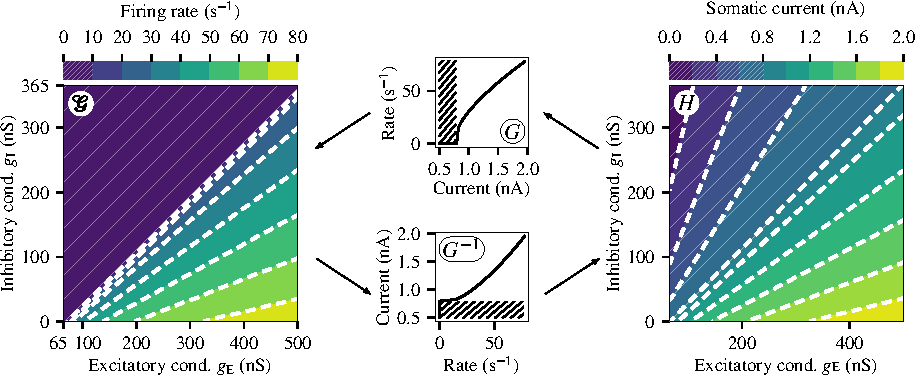
\includegraphics{media/two_compartment_response_curve.pdf}
	\caption{Illustration of the idea of converting a multivariate response function $\mathcal{G}(g_\mathrm{E}, g_\mathrm{I})$ into a synaptic nonlinearity model $H$ by applying the inverse $G^{-1}$ if a simple neural response function. The functions are ill-defined for zero output rates (hatched regions).}
	\label{fig:two_compartment_response_curve}
\end{figure}

\subsection{Computing Nonlinear Multivariate Functions}

\begin{figure}
	\begin{subfigure}{0.33\textwidth}%
		\centering%
		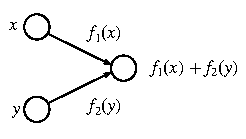
\includegraphics{media/network_a.pdf}%
		\caption{Single layer network}%
		\label{fig:network_a}%
	\end{subfigure}%
	\begin{subfigure}{0.33\textwidth}%
		\centering%
		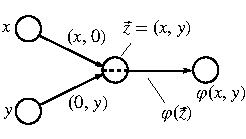
\includegraphics{media/network_c.pdf}%
		\caption{Two-layer network}%
		\label{fig:network_c}%
	\end{subfigure}%
	\begin{subfigure}{0.33\textwidth}%
		\centering%
		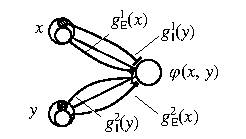
\includegraphics{media/network_d.pdf}%
		\caption{Dendritic computation}%
		\label{fig:network_d}%
	\end{subfigure}%
	\caption{Network architectures for computing multivariate functions. \textbf{(a)} If the input variables are represented in different neuron populations, we can only compute a linear combination of functions of these individual variables. \textbf{(b)} In a \enquote{two-layer network} with an intermediate representation, we can compute arbitrary functions of the two variables. \textbf{(c)} Dendritic computation allows us to compute nonlinear multivariate functions by exploiting synaptic nonlinearities.}
	\label{fig:networks}
\end{figure}

\begin{table}
	\caption{Exploring dendritic computation for the three networks in \cref{fig:networks}. Given values are the average normalised RMSE over 256 experiments with 100 neruons per population (200 in the intermediate population for setup \textbf{(b)}). Maximum firing rates between \SIrange{50}{100}{\hertz}. See \cite{stockel2019passive} for details.}
	\label{tbl:result_table}
	\centering
	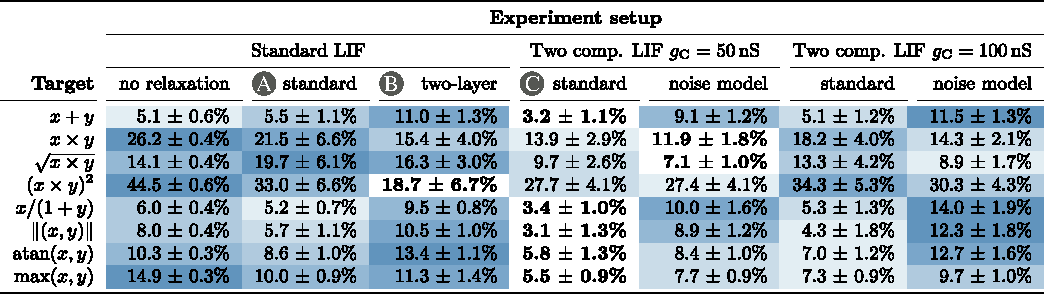
\includegraphics[width=\textwidth]{media/result_table.pdf}
\end{table}

At the beginning of this lecture we noted that we should refrain from adding complexity to the NEF for complexity's sake, and instead think about the role of biological detail in terms of the computation, behaviour, or function that is being performed. So, why should we care about incorporating a more complex synapse model into the NEF?

The answer is that by taking the nonlinear effects in the synapses, or, the \enquote{dendritic} region of the neuron into account, we can use this detail to compute more complex functions in simple networks. This is also known as \enquote{dendritic computation} \cite{london2005dendritic} and is implemented in \texttt{nengo-bio}.

Remember that it is not possible to compute a nonlinear, multivariate function such as multiplication if the inputs are not represented in the same pre-population. A network such as \cref{fig:network_a} cannot compute the product of two numbers, whereas the network in \cref{fig:network_c} can.

Using the nonlinearity model $H$ from \cref{eqn:model_H} for the two-compartment neuron model with conductance-based synapses in \cref{fig:neuron_model}, we can compute multiplication with a relatively small error over the domain $(x, y) \in [0, 1]^2$, as well as a wide variety of other nonlinear multivariate functions. \Cref{tbl:result_table} shows the results from an experiment demonstrating that dendritic computation can even be better than a two-layer network for a wide variety of functions. See \cite{stockel2019passive} for more detail.

\printbibliography

\end{document}

